\chapter{Design}
\section{Overall Architecture}
It was clear from the outset that the server and client portions of the application should be developed independently. The two sections would also be ran independently of each other on different machines. To keep within the time scales of the project only one instance of the server will be running at any time. Multiple servers and load balancing would be ideal but not necessary at this time. The server was written in Python to be run on any compatible server. The client uses Java and designed to run on Android devices, the client then connects directly to the server using PUSH technology.

Nothing radical has been altered about the overall architecture from the progress report. It has simply been expanded while implementing new features.

\section{Data Structures}

\section{Class Diagram}
The class diagram for the client portion of the project can be found in Appendix \ref{ap_class}. The servers architecture is considerably simpler and a diagram is not included in this report.

\section{Use Case Diagram}

\begin{figure}[H]
  \centering
   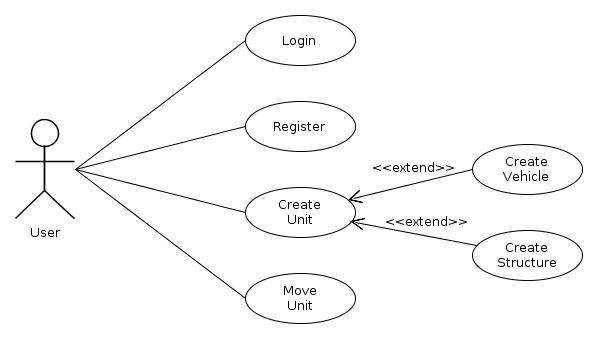
\includegraphics[width=0.8\textwidth]{Images/diagrams/use.png}
  \caption{Use case diagram}
  \label{fig:use}
\end{figure}




\subsection{Language}
Developing applications for the Android OS restricts the language choice to just Java combined with an Android framework. This results in code written with Java syntax but are not entirely synonymous with Java. Code is converted from Java Virtual Machine (JVM) compatible code to code that can be run by Dalvik, the virtual machine used by Android. This conversion optimizes the code to be run on devices with limited memory and processing power.

For the server portion of the application it was important to choose a language that would aid in the rapid development methodology outlined for the project. Python is a general purpose high-level programming language that has a relatively small learning curve as well as some personnel background knowledge. It is designed with the express purpose of being highly readable by forcing well formatted code and using English keywords. 

As the chosen hardware for the server is limited in processing power and memory it is important keep overheads to a minimum, which Python does fairly well. If Java had been used a much more powerful server would have been needed to support the same number of processes due to the overheads introduced by the JVM. However there would have been a number of advantages to using the same language as the client. These include a greater understanding of the language as it is used more extensively but more importantly would be code reuse. The client and server both perform many of the same procedures and could have sped up development time and increased accuracy and interoperability as the same packages could have been utilized.

The server also required a persistent data store to keep an overview of the users and units between downtime or server migration. The requirements specified matched closely to those given when choosing Python as the programming language. 

\begin{itemize}
\item Non-proprietary
\item Simple, zero-configuration database
\item Relational makes things easy
\item Lightweight
\item Previous knowledge of SQL makes that a preferable language of choice
\item Simple python implementation.
\end{itemize}

A nice looking option was KirbyBase\footnote{http://wiki.python.org/moin/KirbyBase} it matched all of the requirements and being purely python based was a plus. It is a flat-file database so was simple to configure and lightweight, it also had the flexibility of running both as part of an application or in a client-server configuration. Unfortunately development stopped in 2006 and the libraries website has since been taken off-line.

MongoDB\footnote{http://www.mongodb.org/} would have also been a nice solution as it supports a large proportion of the requirements and some other features ideal for this project. Unlike other options it is a NoSQL\footnote{http://www.10gen.com/nosql} database which is an entirely different approach to database design than that of the standard relational database. This would have required considerably more investment of time to learn this new style of working. The main draw to MongoDB is that it offers geospatial indexing and queries. This allows the complex calculations of querying coordinates on a sphere could be handled directly by the DBMS.

The chosen SQLite solution has one long term problem that comes with not being able to run a client-server configuration. Thus restricting the application to a single server. As the popularity and interest in the game increases so would the demand on the server meaning that a more complex, distributed server model would be needed. This is outside of the scope of the current project so this was deemed to be an acceptable compromise.

\section{User Interface}
When developing any application for a small form factor it is important to consider how the user interface can be minimized, and to not clutter the display making precise controls difficult. This is especially important when trying to fit all the functionality of a \gls{rts} game within the small form factor of a mobile device. To get around this problem only the essential controls will be included with only a portion of these being accessible from the main game screen.

\begin{figure}[H]
\centering
\begin{minipage}{.5\textwidth}
  \centering
  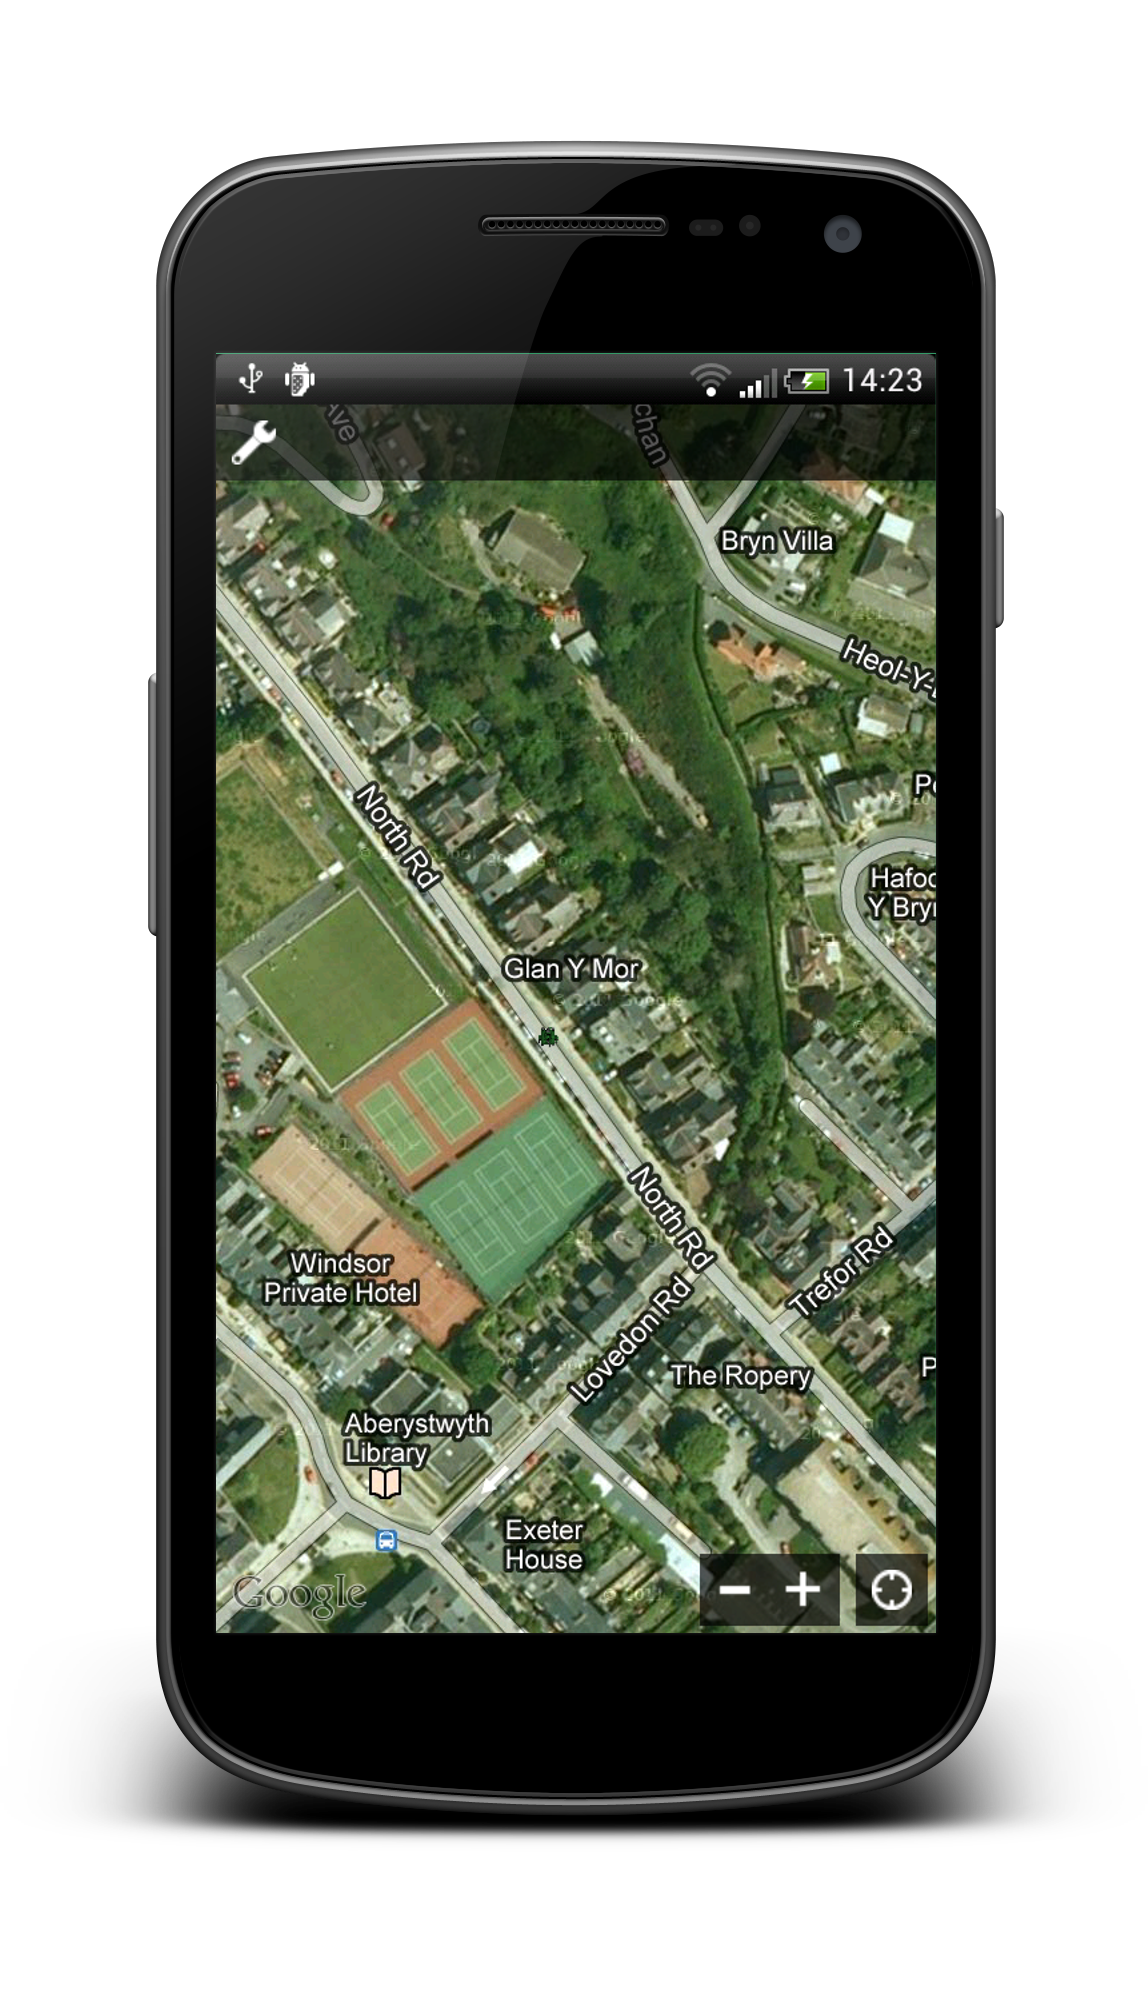
\includegraphics[width=.4\linewidth]{Images/maps-google.png}
  \captionof{figure}{Insert design of game map}
  \label{fig:test1}
\end{minipage}%
\begin{minipage}{.5\textwidth}
  \centering
  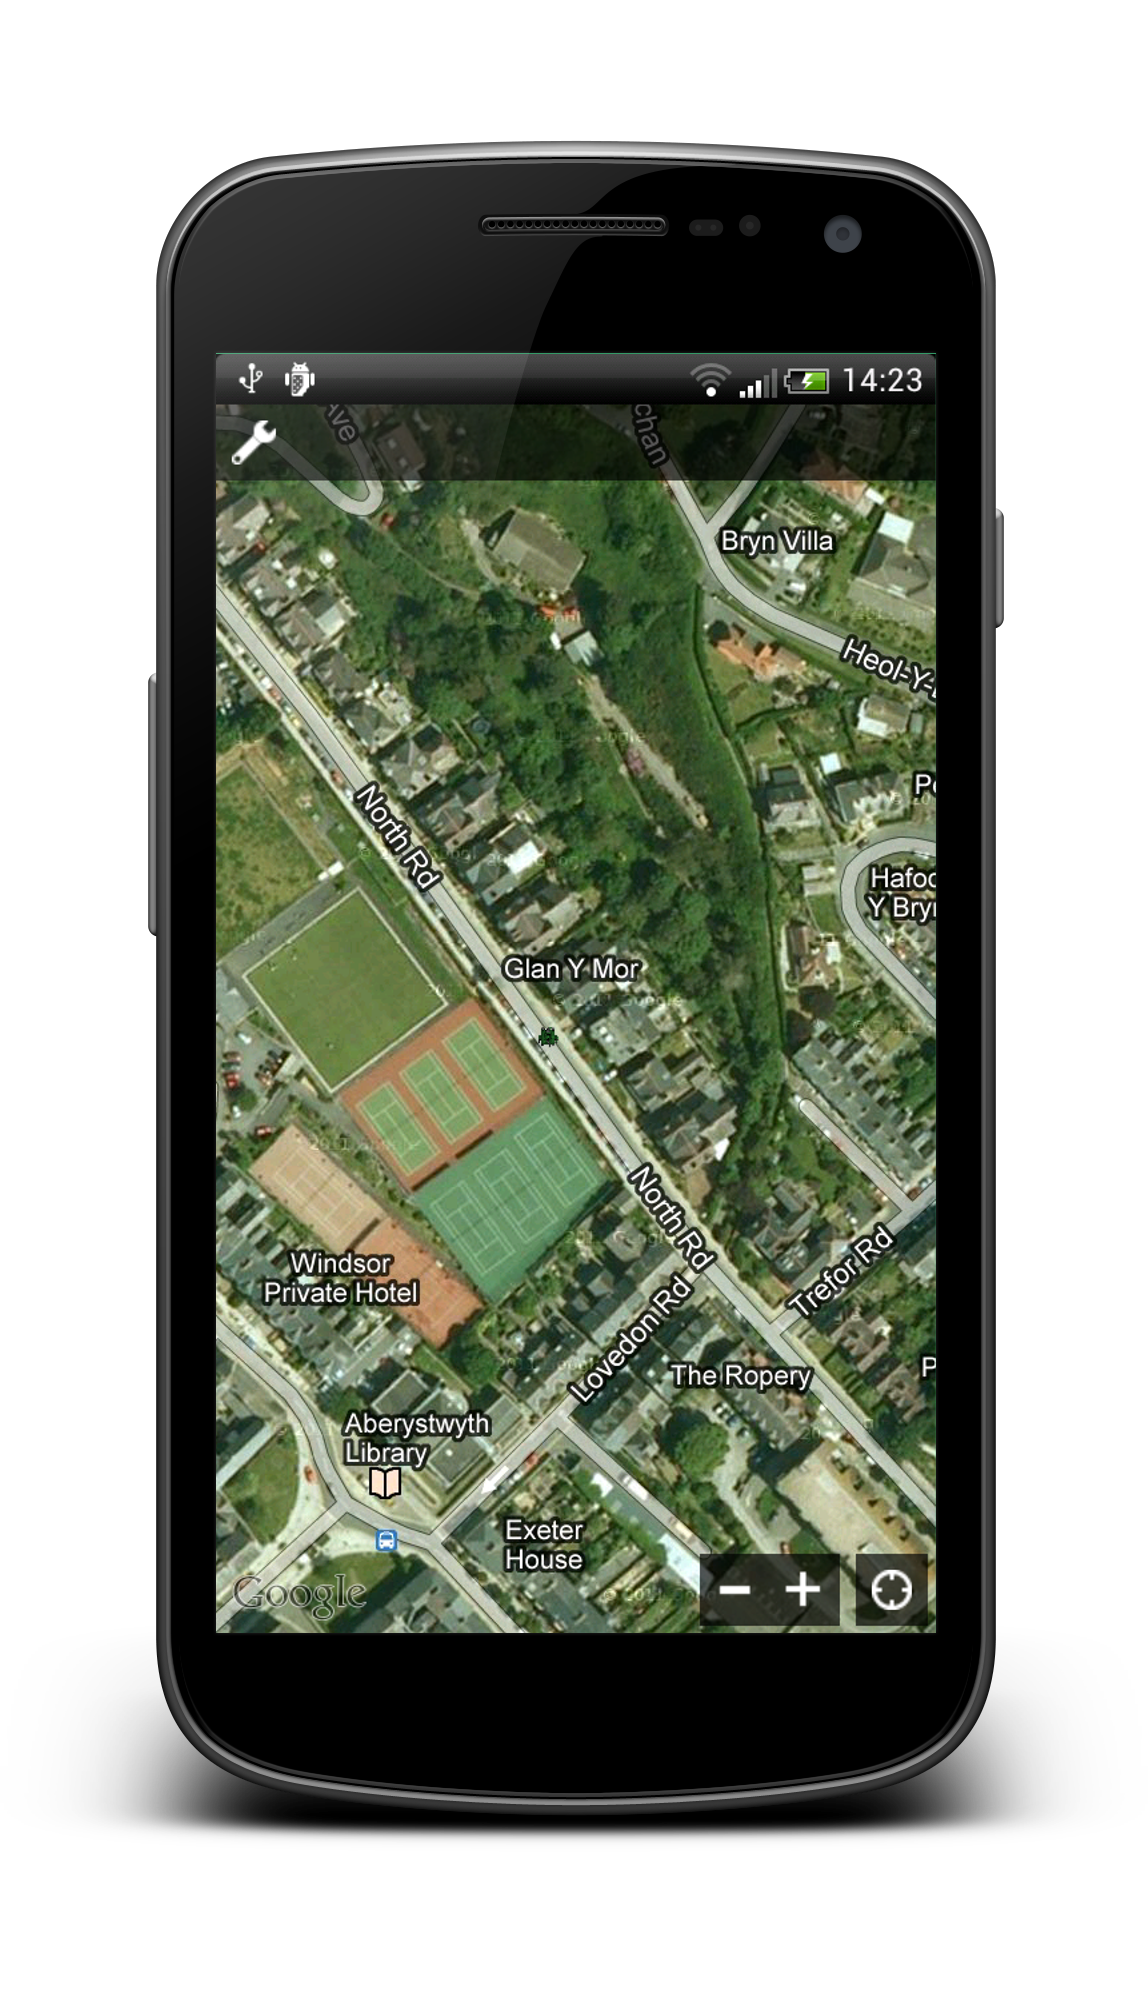
\includegraphics[width=.4\linewidth]{Images/maps-google.png}
  \captionof{figure}{Insert design of game map menu}
  \label{fig:test2}
\end{minipage}
\end{figure}

 Figure \ref{fig:test2}

